% =============================================================================
%  Quadratic Assignment Problem — CSE 462 Final Presentation
%  March 2026
% =============================================================================
\documentclass[aspectratio=169,11pt]{beamer}

% ── Packages ─────────────────────────────────────────────────────────────────
\usepackage[utf8]{inputenc}
\usepackage[T1]{fontenc}
\usepackage{amsmath,amssymb,mathtools}
\usepackage{tikz}
\usetikzlibrary{arrows.meta,positioning,calc,shapes.geometric,matrix,fit,decorations.pathreplacing}
\usepackage{pgfplots}
\pgfplotsset{compat=1.18}
\usepackage{graphicx}
\graphicspath{{plots/}}
\usepackage{booktabs}
\usepackage{colortbl}
\usepackage{multicol}
\usepackage{listings}
\usepackage{hyperref}

% ── Theme & Colors ───────────────────────────────────────────────────────────
\usetheme{Madrid}
\useinnertheme{rounded}

\definecolor{PrimaryBlue}{HTML}{133463}
\definecolor{Teal}{HTML}{007B8C}
\definecolor{Gold}{HTML}{DAA520}
\definecolor{AlertRed}{HTML}{B43737}
\definecolor{LightBG}{HTML}{E8F0F8}

\setbeamercolor{palette primary}{bg=PrimaryBlue,fg=white}
\setbeamercolor{palette secondary}{bg=Teal,fg=white}
\setbeamercolor{palette tertiary}{bg=PrimaryBlue,fg=white}
\setbeamercolor{palette quaternary}{bg=PrimaryBlue,fg=white}
\setbeamercolor{structure}{fg=PrimaryBlue}
\setbeamercolor{titlelike}{fg=white,bg=PrimaryBlue}
\setbeamercolor{frametitle}{fg=white,bg=PrimaryBlue}
\setbeamercolor{block title}{bg=Teal,fg=white}
\setbeamercolor{block body}{bg=LightBG,fg=black}
\setbeamercolor{block title alerted}{bg=AlertRed,fg=white}
\setbeamercolor{block body alerted}{bg=LightBG,fg=black}
\setbeamercolor{block title example}{bg=Gold,fg=black}
\setbeamercolor{block body example}{bg=LightBG,fg=black}
\setbeamercolor{item}{fg=Teal}
\setbeamercolor{footline}{fg=PrimaryBlue}

\setbeamertemplate{footline}[frame number]
\setbeamertemplate{navigation symbols}{}

% ── Metadata ─────────────────────────────────────────────────────────────────
\title[QAP]{Quadratic Assignment Problem}
\subtitle{Definitions, NP-Hardness, Algorithms, and Experiments}
\author[Group 1]{%
  Md.\ Jakaria Hossain~(2005026) \and
  Musa Tur Farazi~(2005038) \and
  Md.\ As-Aid Rahman~(2005039) \and
  MD Sajid Mostafiz Noor~(2005051) \and
  Tausif Rashid~(2005052) \and
  Awesh Islam~(2005054)}
\institute[CSE462]{CSE 462 --- Algorithm Engineering Lab}
\date{March 2026}

% ── Convenience Macros ───────────────────────────────────────────────────────
\newcommand{\pimap}{\pi}
\newcommand{\Sn}{S_n}
\newcommand{\BigO}{\mathcal{O}}
\newcommand{\reference}[1]{\hfill{\scriptsize\textcolor{gray}{#1}}}

% =============================================================================
\begin{document}

% ─── Slide 1: Title ─────────────────────────────────────────────────────────
{
\setbeamertemplate{footline}{}
\begin{frame}[plain]
\vfill
\begin{center}
  \begin{beamercolorbox}[wd=\textwidth,sep=12pt,center]{titlelike}
    \usebeamerfont{title}\inserttitle\\[6pt]
    \usebeamerfont{subtitle}\insertsubtitle
  \end{beamercolorbox}
  \vspace{1.2em}
  {\small
  \begin{tabular}{ccc}
  Md.\ Jakaria Hossain & Musa Tur Farazi & Md.\ As-Aid Rahman\\
  (2005026) & (2005038) & (2005039)\\[6pt]
  MD Sajid Mostafiz Noor & Tausif Rashid & Awesh Islam\\
  (2005051) & (2005052) & (2005054)
  \end{tabular}
  }
  \vspace{1.2em}

  \textbf{CSE462 --- Algorithm Engineering Sessional}\\[4pt]
  March 2026
\end{center}
\vfill
\end{frame}
}

% ─── Slide 2: Agenda ────────────────────────────────────────────────────────
\begin{frame}{Agenda}
\begin{enumerate}\setlength\itemsep{10pt}
  \item \textbf{Problem Definition} --- Koopmans--Beckmann formulation \& variants
  \item \textbf{Complexity Theory} --- NP-Hardness via two reductions
  \item \textbf{Algorithm Landscape} --- Exact, approximation \& metaheuristic families
  \item \textbf{Chosen Algorithms} --- Branch-and-Bound \& Tabu Search
  \item \textbf{Proposed Modifications} --- Greedy UB, LB-Ordered DFS, Reactive Tenure, Diversification
  \item \textbf{Experimental Results} --- Runtime, solution quality, and scalability
\end{enumerate}
\end{frame}

% =============================================================================
%  PART 1: Problem Definition
% =============================================================================

% ─── Slide 3: Motivation — Core Modeling Idea ────────────────────────────────
\begin{frame}{Motivation --- Core Idea}
\begin{columns}[T]
\column{0.48\textwidth}
\centering
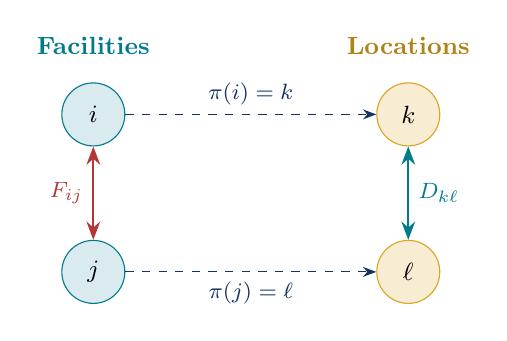
\begin{tikzpicture}[
    fnode/.style={circle,draw=Teal,fill=Teal!15,minimum size=8mm,font=\small},
    lnode/.style={circle,draw=Gold,fill=Gold!20,minimum size=8mm,font=\small},
    >=Stealth
  ]
  % Facilities
  \node[fnode] (fi) at (0,1.5) {$i$};
  \node[fnode] (fj) at (0,-0.5) {$j$};
  % Locations
  \node[lnode] (lk) at (4,1.5) {$k$};
  \node[lnode] (ll) at (4,-0.5) {$\ell$};
  % Flow
  \draw[<->,thick,AlertRed] (fi) -- node[left,font=\footnotesize]{$F_{ij}$} (fj);
  % Distance
  \draw[<->,thick,Teal] (lk) -- node[right,font=\footnotesize]{$D_{k\ell}$} (ll);
  % Assignments
  \draw[->,dashed,PrimaryBlue] (fi) -- node[above,font=\footnotesize]{$\pi(i)=k$} (lk);
  \draw[->,dashed,PrimaryBlue] (fj) -- node[below,font=\footnotesize]{$\pi(j)=\ell$} (ll);
  % Labels
  \node[above=4pt,font=\small\bfseries,Teal] at (0,2) {Facilities};
  \node[above=4pt,font=\small\bfseries,Gold!80!black] at (4,2) {Locations};
\end{tikzpicture}

\column{0.50\textwidth}
\textbf{Key quantities:}
\begin{itemize}
  \item $F_{ij}$: \alert{flow} between facilities $i$ and $j$
  \item $D_{k\ell}$: \alert{distance} between locations $k$ and $\ell$
  \item $\pi$: assignment (bijection) of facilities to locations
\end{itemize}
\vspace{6pt}
\begin{block}{Total Cost}
\[
  \text{Cost}(\pi) = \sum_{i=1}^{n}\sum_{j=1}^{n} F_{ij}\cdot D_{\pi(i),\pi(j)}
\]
\end{block}
Minimize the total weighted distance!
\end{columns}
\end{frame}

% ─── Slide 4: Formal Definition (Koopmans–Beckmann) ─────────────────────────
\begin{frame}{Formal Definition (Koopmans--Beckmann, 1957)}
\textbf{Given:}
\begin{itemize}
  \item Flow matrix $F \in \mathbb{R}^{n\times n}$, \quad Distance matrix $D \in \mathbb{R}^{n\times n}$
  \item Optionally, linear cost matrix $C \in \mathbb{R}^{n\times n}$
\end{itemize}
\vspace{8pt}
\begin{block}{Objective}
\[
  \min_{\pi\in\Sn}\;\;
  \underbrace{\sum_{i=1}^{n}\sum_{j=1}^{n} F_{ij}\,D_{\pi(i),\pi(j)}}_{\text{Quadratic Pair Cost}}
  \;+\;
  \underbrace{\sum_{i=1}^{n} C_{i,\pi(i)}}_{\text{Linear Cost}}
\]
\end{block}
\vspace{4pt}
\begin{itemize}
  \item $\Sn$: set of all permutations of $\{1,\dots,n\}$ \quad ($|\Sn|=n!$)
  \item When $C=0$: Homogeneous QAP
\end{itemize}
\reference{Koopmans \& Beckmann, \emph{Econometrica}, 1957}
\end{frame}

% ─── Slide 5: Trace Formulation ─────────────────────────────────────────────
\begin{frame}{Trace Formulation}
Let $\Pi_n$ be the set of all $n\times n$ \alert{permutation matrices}.
\vspace{6pt}
\begin{block}{Trace Form}
\[
  \min_{P \in \Pi_n}\;\;
  \mathrm{tr}\!\bigl(F\,P\,D\,P^{\!\top}\bigr)
  \;+\;
  \mathrm{tr}\!\bigl(C^{\!\top} P\bigr)
\]
\end{block}
\vspace{6pt}
\centering
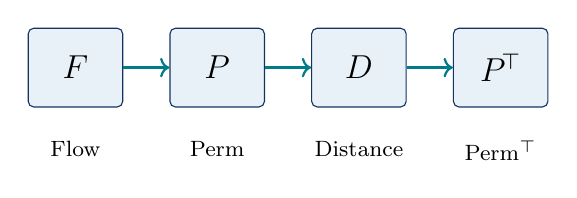
\begin{tikzpicture}[
    box/.style={draw=PrimaryBlue,fill=LightBG,minimum width=12mm,minimum height=10mm,
                font=\large\bfseries,rounded corners=2pt}
  ]
  \node[box] (F) at (0,0)   {$F$};
  \node[box] (P) at (1.8,0) {$P$};
  \node[box] (D) at (3.6,0) {$D$};
  \node[box] (PT)at (5.4,0) {$P^{\!\top}$};
  \draw[->,thick,Teal] (F.east) -- (P.west);
  \draw[->,thick,Teal] (P.east) -- (D.west);
  \draw[->,thick,Teal] (D.east) -- (PT.west);
  \node[below=6pt,font=\footnotesize] at (0,-.6) {Flow};
  \node[below=6pt,font=\footnotesize] at (1.8,-.6) {Perm};
  \node[below=6pt,font=\footnotesize] at (3.6,-.6) {Distance};
  \node[below=6pt,font=\footnotesize] at (5.4,-.6) {Perm$^\top$};
\end{tikzpicture}
\vspace{4pt}

Equivalent to Koopmans--Beckmann when $P$ encodes $\pi$.
\end{frame}

% ─── Slide 6: 0-1 Quadratic Program ─────────────────────────────────────────
\begin{frame}{0--1 Quadratic Integer Program}
\textbf{Binary variable:}\quad $x_{ik}\in\{0,1\}$: facility $i$ assigned to location $k$.

\vspace{6pt}
\begin{block}{Assignment Constraints}
\[
  \sum_{k=1}^{n} x_{ik} = 1 \;\;\forall\, i
  \qquad\qquad
  \sum_{i=1}^{n} x_{ik} = 1 \;\;\forall\, k
\]
\end{block}

\begin{block}{Objective}
\[
  \min \;\;
  \sum_{i=1}^{n}\sum_{j=1}^{n}\sum_{k=1}^{n}\sum_{\ell=1}^{n}
  F_{ij}\,D_{k\ell}\,x_{ik}\,x_{j\ell}
  \;+\;
  \sum_{i=1}^{n}\sum_{k=1}^{n} C_{ik}\,x_{ik}
\]
\end{block}

\begin{itemize}
  \item $n^2$ binary variables, $2n$ equality constraints
  \item Quadratic terms $x_{ik}\,x_{j\ell}$ make this \alert{non-convex}
\end{itemize}
\end{frame}

% =============================================================================
%  PART 2: Complexity Theory
% =============================================================================

% ─── Slide 7: Decision Problem ──────────────────────────────────────────────
\begin{frame}{QAP Decision Problem (QAP-DEC)}
\begin{block}{Instance}
Matrices $F,D\in\mathbb{R}^{n\times n}$ and a cost bound $B\in\mathbb{R}$.
\end{block}
\begin{block}{Question}
Does there exist $\pi\in\Sn$ such that $\mathrm{Cost}(\pi)\le B$\,?
\end{block}
\vspace{8pt}
\begin{alertblock}{Lemma: QAP-DEC $\in$ NP}
\textbf{Certificate:} A permutation $\pi$.\\
\textbf{Verification:} Compute $\mathrm{Cost}(\pi)=\sum_{i}\sum_{j}F_{ij}D_{\pi(i),\pi(j)}$ in $\BigO(n^2)$ time
and check $\mathrm{Cost}(\pi)\le B$.
\end{alertblock}
\end{frame}

% ─── Slide 8: Complexity Overview ────────────────────────────────────────────
\begin{frame}{Complexity Overview}
\begin{block}{Theorem}
\textbf{QAP-DEC is NP-Complete.}  Therefore the optimization QAP is \alert{NP-Hard}.
\end{block}
\vspace{6pt}
\centering
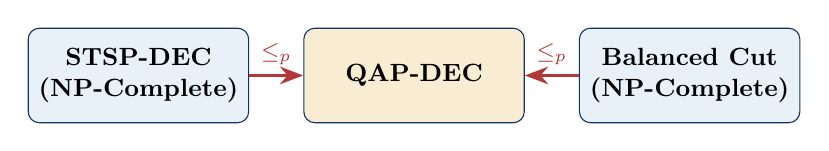
\begin{tikzpicture}[
    probbox/.style={draw=PrimaryBlue,fill=LightBG,rounded corners=4pt,
                    minimum width=28mm,minimum height=12mm,align=center,font=\small\bfseries},
    >=Stealth
  ]
  \node[probbox] (stsp) at (-3.5,0) {STSP-DEC\\(NP-Complete)};
  \node[probbox,fill=Gold!20] (qap)  at (0,0) {QAP-DEC};
  \node[probbox] (bcut) at (3.5,0)  {Balanced Cut\\(NP-Complete)};
  \draw[->,very thick,AlertRed] (stsp) -- node[above,font=\footnotesize]{$\le_p$} (qap);
  \draw[->,very thick,AlertRed] (bcut) -- node[above,font=\footnotesize]{$\le_p$} (qap);
\end{tikzpicture}
\vspace{8pt}

\textbf{Recall:} Symmetric Travelling Salesman Problem (STSP)\\
  \vspace{20pt}
Given cities with symmetric distances, find a tour of cost $\le L$.
\reference{Sahni \& Gonzalez, \emph{JACM}, 1976}
\end{frame}

% ─── Slide 9: Reduction 1: STSP ≤_p QAP ─────────────────────────────────────
\begin{frame}{Reduction 1: STSP $\le_p$ QAP}
\textbf{Given:} STSP instance with distance matrix $D^{\text{TSP}}\in\mathbb{R}^{n\times n}$ and bound $L$.

\vspace{6pt}
\begin{block}{Construction (polynomial time)}
\begin{enumerate}
  \item Set $D := D^{\text{TSP}}$ \quad (same distance matrix)
  \item Set $B := 2L$ \quad (QAP cost bound)
  \item Construct $F$ as the \alert{adjacency matrix of an $n$-cycle}
\end{enumerate}
\end{block}
\vspace{4pt}
\begin{itemize}
  \item Reduction runs in $\BigO(n^2)$ time
  \item $F$ has exactly $2n$ ones (each vertex connected to two neighbors)
  \item Key idea: the QAP cost with cycle flow counts each tour edge \alert{twice}
\end{itemize}
\reference{Sahni \& Gonzalez, 1976}
\end{frame}

% ─── Slide 10: Constructing Matrix F ─────────────────────────────────────────
\begin{frame}{Constructing the Cycle Flow Matrix $F$}
\[
  F_{ij} = \begin{cases}
    1 & \text{if } |i-j|=1 \text{ or } \{i,j\}=\{1,n\}\\
    0 & \text{otherwise}
  \end{cases}
\]
\vspace{2pt}
\begin{columns}[c]
\column{0.52\textwidth}
\centering
\textbf{Example} ($n=6$):\\[4pt]
$F = \begin{pmatrix}
  \cellcolor{Teal!20}0 & \cellcolor{Gold!30}1 & 0 & 0 & 0 & \cellcolor{Gold!30}1\\
  \cellcolor{Gold!30}1 & \cellcolor{Teal!20}0 & \cellcolor{Gold!30}1 & 0 & 0 & 0\\
  0 & \cellcolor{Gold!30}1 & \cellcolor{Teal!20}0 & \cellcolor{Gold!30}1 & 0 & 0\\
  0 & 0 & \cellcolor{Gold!30}1 & \cellcolor{Teal!20}0 & \cellcolor{Gold!30}1 & 0\\
  0 & 0 & 0 & \cellcolor{Gold!30}1 & \cellcolor{Teal!20}0 & \cellcolor{Gold!30}1\\
  \cellcolor{Gold!30}1 & 0 & 0 & 0 & \cellcolor{Gold!30}1 & \cellcolor{Teal!20}0
\end{pmatrix}$

\column{0.44\textwidth}
\centering
\textbf{Cycle graph:}\\[6pt]
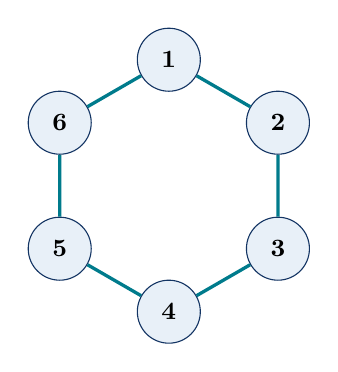
\begin{tikzpicture}[
    cnode/.style={circle,draw=PrimaryBlue,fill=LightBG,minimum size=8mm,font=\small\bfseries},
  ]
  \foreach \i/\a in {1/90,2/30,3/-30,4/-90,5/-150,6/150} {
    \node[cnode] (n\i) at (\a:1.6) {\i};
  }
  \draw[very thick,Teal] (n1)--(n2)--(n3)--(n4)--(n5)--(n6)--(n1);
\end{tikzpicture}
\end{columns}
\end{frame}

% ─── Slide 11: Key Lemma and Proof ──────────────────────────────────────────
% ─── Slide 11: Key Lemma and Proof ──────────────────────────────────────────
\begin{frame}[shrink=5]{Key Lemma}
\begin{alertblock}{Lemma}
For every permutation $\pi\in\Sn$:\;
$C_{\text{QAP}}(\pi) = 2\cdot\mathrm{TourLen}(\pi)$
\end{alertblock}
\vspace{2pt}
\begin{columns}[T]
\column{0.4\textwidth}
\textbf{Visualized ($n\!=\!4$, $\pi=\mathrm{id}$):}
\begin{center}
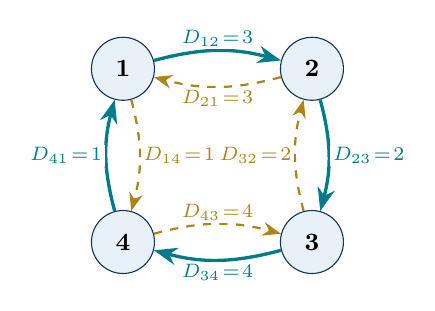
\begin{tikzpicture}[
    cnode/.style={circle,draw=PrimaryBlue,fill=LightBG,minimum size=8mm,font=\small\bfseries},
    elbl/.style={font=\scriptsize,fill=white,inner sep=1pt},
    >=Stealth,
  ]
  % Nodes in cycle order (wide spacing for label clarity)
  \node[cnode] (n1) at (0,2.2) {1};
  \node[cnode] (n2) at (2.4,2.2) {2};
  \node[cnode] (n3) at (2.4,0) {3};
  \node[cnode] (n4) at (0,0) {4};
  % Forward edges (solid, Teal) — labels on outer side
  \draw[very thick,Teal,->] (n1) to[bend left=15] node[elbl,above]{$D_{12}\!=\!3$} (n2);
  \draw[very thick,Teal,->] (n2) to[bend left=15] node[elbl,right]{$D_{23}\!=\!2$} (n3);
  \draw[very thick,Teal,->] (n3) to[bend left=15] node[elbl,below]{$D_{34}\!=\!4$} (n4);
  \draw[very thick,Teal,->] (n4) to[bend left=15] node[elbl,left]{$D_{41}\!=\!1$} (n1);
  % Backward edges (dashed, Gold) — labels on inner side
  \draw[thick,Gold!80!black,->,dashed] (n2) to[bend left=15] node[elbl,below]{$D_{21}\!=\!3$} (n1);
  \draw[thick,Gold!80!black,->,dashed] (n3) to[bend left=15] node[elbl,left]{$D_{32}\!=\!2$} (n2);
  \draw[thick,Gold!80!black,->,dashed] (n4) to[bend left=15] node[elbl,above]{$D_{43}\!=\!4$} (n3);
  \draw[thick,Gold!80!black,->,dashed] (n1) to[bend left=15] node[elbl,right]{$D_{14}\!=\!1$} (n4);
\end{tikzpicture}
\end{center}
\vspace{-2pt}
{\scriptsize \textcolor{Teal}{Forward} + \textcolor{Gold!80!black}{backward} on each cycle edge\\
$C_{\text{QAP}} = (3\!+\!3)+(2\!+\!2)+(4\!+\!4)+(1\!+\!1) = 20 = 2\times 10$}

\column{0.57\textwidth}
\textbf{Proof sketch:}
\begin{align*}
  C_{\text{QAP}}(\pi)
  &= \sum_{i}\sum_{j} F_{ij}\,D_{\pi(i),\pi(j)} \\
  &= \sum_{\{i,j\}:\,F_{ij}=1} \bigl(D_{\pi(i),\pi(j)}+D_{\pi(j),\pi(i)}\bigr) \\
  &= 2\sum_{e\in\text{cycle}} D_{\pi(\text{endpoints of }e)} \\
  &= 2\cdot\mathrm{TourLen}(\pi)
\end{align*}
Uses symmetry $D_{kl}=D_{lk}$ and the fact that each cycle edge contributes a forward \emph{and} backward term.
\end{columns}
\end{frame}


% ─── Slide 12: Correctness ──────────────────────────────────────────────────
\begin{frame}{Correctness of Reduction 1}
\begin{block}{Forward direction: STSP YES $\Rightarrow$ QAP YES}
If $\pi^*$ is a tour with $\mathrm{TourLen}(\pi^*)\le L$, then
\[
  C_{\text{QAP}}(\pi^*) = 2\cdot\mathrm{TourLen}(\pi^*) \le 2L = B \quad\checkmark
\]
\end{block}
\begin{block}{Backward direction: QAP YES $\Rightarrow$ STSP YES}
If $\pi$ satisfies $C_{\text{QAP}}(\pi)\le B=2L$, then
\[
  \mathrm{TourLen}(\pi) = \tfrac{1}{2}\,C_{\text{QAP}}(\pi) \le L \quad\checkmark
\]
\end{block}
\vspace{4pt}
\begin{alertblock}{Result}
Since STSP-DEC is NP-Complete and STSP $\le_p$ QAP, we conclude \textbf{QAP-DEC is NP-Hard}.
\end{alertblock}
\end{frame}

% ─── Slide 13: Reduction 2: Balanced Cut → QAP ──────────────────────────────
\begin{frame}{Reduction 2: Balanced Cut $\le_p$ QAP}
\textbf{Balanced Cut (Fixed-Size Cut):}
Given graph $G=(V,E,w)$ and integer $K$, is there a partition
$(S,V\!\setminus\!S)$ with $|S|=\lfloor n/2\rfloor$ and $\mathrm{cut}(S)\le K$?

\vspace{6pt}
\begin{block}{Construction}
\begin{itemize}
  \item $F_{uv} := w_{uv}$ \quad (edge weights become flows)
  \item Locations split into two groups $A$ and $B$, each of size $\lfloor n/2\rfloor$
  \item Distance matrix:
    \[
      D_{k\ell} = \begin{cases}
        0 & \text{if } k,\ell \text{ in same group}\\
        1 & \text{if } k,\ell \text{ in different groups}
      \end{cases}
    \]
  \item QAP bound $B := 2K$
\end{itemize}
\end{block}
\reference{Garey \& Johnson, 1979}
\end{frame}

% ─── Slide 14: Balanced Cut Correctness ──────────────────────────────────────

% ─── Slide 14a: Balanced Cut — Lemma & Proof ─────────────────────────────────
\begin{frame}{Balanced Cut: Lemma \& Proof}

\begin{alertblock}{Key Lemma}
\[
  C_{\text{QAP}}(\pi) = 2\cdot\mathrm{Cut}\bigl(S(\pi)\bigr)
  \qquad\text{where } S(\pi)=\{u : \pi(u)\in A\}
\]
\end{alertblock}

\vspace{2pt}
\begin{columns}[T]

%--- Left column: Proof steps ---%
\column{0.45\textwidth}
\textbf{Proof:}
\begin{itemize}
  \item<2-> \textbf{Step 1:} Each term
    $F_{uv}\,D_{\pi(u),\pi(v)} = w_{uv}\cdot\mathbf{1}[\text{different groups}]$
  \item<3-> \textbf{Step 2:} Sum over all ordered pairs —
    each cut edge $(u,v)$ counted once as $(u,v)$ and once as $(v,u)$.
  \item<4-> \textbf{Step 3:} Therefore
    $C_{\text{QAP}}(\pi)=2\cdot\mathrm{Cut}\bigl(S(\pi)\bigr)$.\;\;$\blacksquare$
\end{itemize}

%--- Right column: TikZ visualisation ---%
\column{0.52\textwidth}
\centering
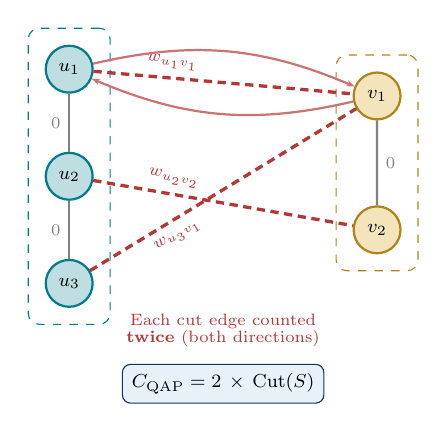
\begin{tikzpicture}[
  vertex/.style={circle, draw, thick, minimum size=7mm, font=\footnotesize\bfseries},
  groupA/.style={vertex, fill=Teal!25, draw=Teal},
  groupB/.style={vertex, fill=Gold!30, draw=Gold!80!black},
  cutedge/.style={very thick, AlertRed, densely dashed},
  inneredge/.style={thick, black!50},
  label/.style={font=\scriptsize\itshape},
  scale=0.85, transform shape
]

% --- Group A (left cloud) ---
\uncover<1->{
  \node[groupA] (a1) at (0,1.6)   {$u_1$};
  \node[groupA] (a2) at (0,0)     {$u_2$};
  \node[groupA] (a3) at (0,-1.6)  {$u_3$};
  % group label
  \node[draw=Teal, rounded corners, dashed, fit=(a1)(a2)(a3),
        inner sep=6pt, label={[Teal,font=\footnotesize]above:Group $A$}] {};
}

% --- Group B (right cloud) ---
\uncover<1->{
  \node[groupB] (b1) at (4.6,1.2)   {$v_1$};
  \node[groupB] (b2) at (4.6,-0.8)  {$v_2$};
  % group label
  \node[draw=Gold!80!black, rounded corners, dashed, fit=(b1)(b2),
        inner sep=6pt, label={[Gold!80!black,font=\footnotesize]above:Group $B$}] {};
}

% --- Inner edges (same group, cost = 0) ---
\uncover<1->{
  \draw[inneredge] (a1) -- node[label,left]{$0$} (a2);
  \draw[inneredge] (a2) -- node[label,left]{$0$} (a3);
  \draw[inneredge] (b1) -- node[label,right]{$0$} (b2);
}

% --- Cut edges (cross-group, cost = w) shown at Step 1 ---
\uncover<2->{
  \draw[cutedge] (a1) -- node[label,above,sloped,AlertRed,pos=0.3]{$w_{u_1 v_1}$} (b1);
  \draw[cutedge] (a2) -- node[label,above,sloped,AlertRed,pos=0.3]{$w_{u_2 v_2}$} (b2);
  \draw[cutedge] (a3) -- node[label,below,sloped,AlertRed,pos=0.3]{$w_{u_3 v_1}$} (b1);
}

% --- Double-counting annotation at Step 2 ---
\uncover<3->{
  \draw[-{Stealth[length=3pt]}, AlertRed!70, thick, bend left=18]
    (a1) to (b1);
  \draw[-{Stealth[length=3pt]}, AlertRed!70, thick, bend left=18]
    (b1) to (a1);
  \node[font=\scriptsize, AlertRed, align=center] at (2.3,-2.3)
    {Each cut edge counted\\[-1pt] \textbf{twice} (both directions)};
}

% --- Final formula annotation at Step 3 ---
\uncover<4->{
  \node[fill=LightBG, draw=PrimaryBlue, rounded corners=3pt,
        font=\footnotesize, inner sep=4pt, align=center] at (2.3,-3.1)
    {$C_{\text{QAP}} = 2\,\times\,\text{Cut}(S)$};
}

\end{tikzpicture}
\end{columns}
\end{frame}

% ─── Slide 14b: Balanced Cut — Conclusion ────────────────────────────────────
\begin{frame}{Balanced Cut: Conclusion}

\begin{block}{Reduction Equivalence}
\begin{itemize}
  \item<2-> \textbf{Forward:}\;
    $\mathrm{Cut}(S)\le K
      \;\Longrightarrow\;
      C_{\text{QAP}}= 2\,\mathrm{Cut}(S) \le 2K = B$
  \item<3-> \textbf{Backward:}\;
    $C_{\text{QAP}}\le 2K
      \;\Longrightarrow\;
      \mathrm{Cut}(S) = \tfrac{1}{2}\,C_{\text{QAP}} \le K$
\end{itemize}
\end{block}

\vspace{6pt}

\uncover<4->{
\begin{center}
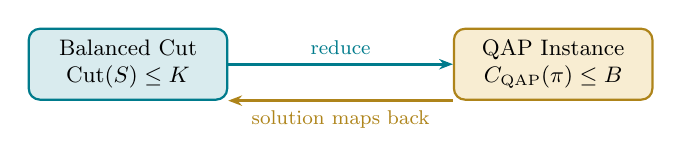
\begin{tikzpicture}[
  box/.style={draw, rounded corners=4pt, thick, minimum width=2.8cm,
              minimum height=1cm, font=\small, align=center},
  arr/.style={-{Stealth[length=5pt]}, very thick},
  scale=0.9, transform shape
]
  \node[box, fill=Teal!15, draw=Teal]       (bc) at (0,0)
    {Balanced Cut\\$\mathrm{Cut}(S)\le K$};
  \node[box, fill=Gold!20, draw=Gold!80!black] (qap) at (6,0)
    {QAP Instance\\$C_{\text{QAP}}(\pi)\le B$};

  \draw[arr, Teal]            (bc.east)  -- node[above, font=\footnotesize]{reduce} (qap.west);
  \draw[arr, Gold!80!black]   (qap.south west) -- node[below, font=\footnotesize]{solution maps back} (bc.south east);
\end{tikzpicture}
\end{center}
}

\vspace{4pt}
\uncover<5->{
\begin{alertblock}{Takeaway}
QAP faithfully encodes \alert{balanced graph partitioning} —
the optimal QAP assignment \emph{is} the optimal balanced cut,
confirming NP-hardness.
\end{alertblock}
}
\end{frame}


% =============================================================================
%  PART 3: Algorithm Landscape
% =============================================================================

% ─── Slide 15: Algorithms─────────────────────────────────────────
\begin{frame}[shrink=5]{Existing Algorithms}
\small
\begin{columns}[T]
\column{0.48\textwidth}
\begin{block}{\centering Exact}
\textbf{Branch-and-Bound}: Enumerate partial assignments, prune via lower bounds.\\
{\scriptsize Gilmore, \emph{SIAM J.}, 1962; Lawler, \emph{Mgmt.\ Sci.}, 1963}\\
{\scriptsize Worst-case $\Omega(n!)$}
\end{block}

\begin{block}{\centering Metaheuristic (Our Focus)}
\textbf{Tabu Search}: Local search with memory to escape local optima.\\
{\scriptsize Taillard, \emph{Parallel Computing}, 1991}\\[2pt]
\textbf{Simulated Annealing}: Accept worse solutions with decreasing probability.\\
{\scriptsize Burkard \& Rendl, \emph{EJOR}, 1984}\\[2pt]
\textbf{Genetic Algorithms}: Population-based evolution with crossover.\\
{\scriptsize Drezner, \emph{INFORMS J.\ Comp.}, 2003}
\end{block}

\column{0.48\textwidth}
\begin{block}{\centering Approximation}
\textbf{LP/SDP Relaxation}: Relax integrality constraints, then round.\\
\textbf{Spectral Bounds}: Eigenvalue-based lower bounds.\\
{\scriptsize Rendl \& Sotirov, \emph{Math.\ Prog.}, 2007}\\
{\scriptsize General QAP is hard to approximate.}
\end{block}

\begin{block}{\centering Randomized}
\textbf{Random Restart}: Run local search from many random starts, keep best.\\[2pt]
\textbf{GRASP}: Greedy randomized construction followed by local search.\\
{\scriptsize Resende et al., \emph{Discrete Appl.\ Math.}, 1996}
\end{block}
\end{columns}

\vspace{4pt}
\centering
{\scriptsize
Survey: Loiola et al., \emph{European J.\ Operational Research}, 176(2), 657--690, 2007.
}
\end{frame}

% =============================================================================
%  PART 4: Chosen Algorithms
% =============================================================================

% ─── Slide 16: Branch-and-Bound ─────────────────────────────────────────────
\begin{frame}{Algorithm 1: Branch-and-Bound}

\begin{columns}[T]

%--- Left column: Algorithm description ---%
\begin{column}{0.43\textwidth}
  \textbf{Search space:} Tree of partial assignments


  \textbf{Node:}
  \begin{itemize}
    \item Fixed set $I_{\text{fix}}$: assigned pairs
    \item Free set $I_{\text{free}}$: unassigned facilities
  \end{itemize}


  \textbf{Branch:}
  \begin{itemize}
    \item Assign next facility $i$ to each free location $k$
    \item Creates one child per available location
  \end{itemize}


  \textbf{Prune:}
  \begin{itemize}
    \item Compute lower bound $\text{LB}(\text{node})$
    \item If $\text{LB}(\text{node}) \geq \text{UB}$ $\Rightarrow$ \alert{cut branch}
  \end{itemize}
\end{column}

%--- Right column: Search tree diagram ---%
\begin{column}{0.53\textwidth}
  \centering
  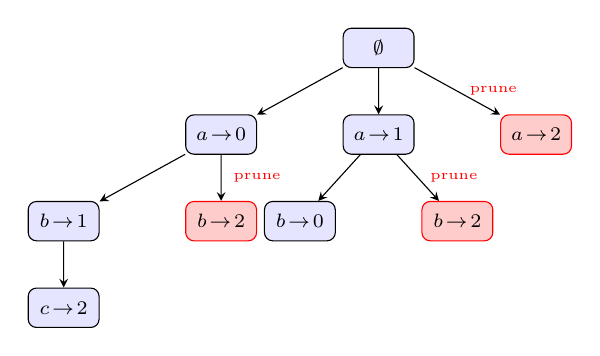
\begin{tikzpicture}[
    every node/.style={
      draw, rounded corners=3pt,
      font=\scriptsize,
      minimum width=.9cm,
      minimum height=0.5cm,
      fill=blue!10
    },
    pruned/.style={fill=red!20, draw=red},
    invisible/.style={fill=white, draw=none},
    level distance=1.1cm,
    sibling distance=2cm,
    edge from parent/.style={draw, -stealth, thin},
    edge from parentx/.style={draw=none},
    label style/.style={draw=none, fill=none, font=\tiny}
  ]

  % Root
  \node (root) {$\emptyset$}
    child {
      node (a0) {$a \!\to\! 0$}
        child {
          node {$b \!\to\! 1$}
            child { node{$c \!\to\! 2$} }
        }
        child {
          node[pruned] {$b \!\to\! 2$}
            edge from parent node[label style, right] {\color{red}\tiny prune}
        }
        child {
          node[invisible] {}
            edge from parent[draw=none]
        }
      edge from parent node[label style, left] {}
    }
    child {
      node (a1) {$a \!\to\! 1$}
        child {
          node {$b \!\to\! 0$}
        }
        child {
          node[pruned] {$b \!\to\! 2$}
            edge from parent node[label style, right] {\color{red}\tiny prune}
        }
    }
    child {
      node[pruned] (a3) {$a \!\to\! 2$}
        edge from parent node[label style, right] {\color{red}\tiny prune}
    };

  \end{tikzpicture}

  \vspace{0.3em}
  {\scriptsize \textcolor{red}{$\blacksquare$}~Pruned \quad
               \textcolor{blue!60!black}{$\blacksquare$}~Explored}
\end{column}

\end{columns}

\end{frame}

% ─── Slide 17: Gilmore–Lawler Lower Bound ────────────────────────────────────
\begin{frame}{Gilmore--Lawler Lower Bound (GLB)}
\textbf{Cost decomposition} at a partial assignment node:
\[
  C(\pi) = \underbrace{C_{\text{fixed}}}_{\text{known}}
  + \underbrace{C_{\text{fixed-free}}}_{\text{partially known}}
  + \underbrace{C_{\text{free-free}}}_{\text{unknown}}
\]

\vspace{6pt}
\begin{block}{Lower Bound via Linear Assignment}
\[
  \mathrm{LB} = C_{\text{fixed}}
  + \min_{x}\sum_{i\in I_{\text{free}}}\sum_{k\in K_{\text{free}}}
    \hat{M}_{ik}\,x_{ik}
  \qquad\text{(LAP)}
\]
\end{block}
\begin{itemize}
  \item $\hat{M}_{ik}$: reduced cost of assigning free facility $i$ to free location $k$
  \item Solved by the \alert{Hungarian Algorithm} in $\BigO(n^3)$
\end{itemize}
\vspace{4pt}
\reference{Gilmore, 1962; Lawler, 1963}
\end{frame}

% ─── Slide 18: B&B & GLB Pseudocode ─────────────────────────────────────────
\begin{frame}{Branch-and-Bound \& GLB --- Pseudocode}
\vspace{-4pt}
\begin{columns}[T]

% --- Left Column: B&B Main Loop ---
\column{0.50\textwidth}
\begin{block}{B\&B Main Loop}
\footnotesize
\vspace{-2pt}
\begin{tabbing}
\hspace{3mm}\=\hspace{3mm}\=\hspace{3mm}\=\hspace{3mm}\=\kill
\textbf{Initialize:} $\mathrm{UB}\leftarrow +\infty$,\; $Q\leftarrow\{\text{Root}\}$\\[2pt]
\textbf{while} $Q\neq\emptyset$ \textbf{do}\\
\> Pop node with smallest LB from $Q$\\
\> \textbf{if} $\mathrm{LB}\ge\mathrm{UB}$: \textbf{continue} \hfill\textit{// Prune}\\
\> \textbf{if} node is complete:\\
\>\> Update $\mathrm{UB}$, $\pi^*$\\
\> \textbf{else}:\\
\>\> Pick unassigned facility $i$\\
\>\> \textbf{for each} free location $k$:\\
\>\>\> Create child (fix $i\!\to\!k$)\\
\>\>\> $\mathrm{LB}(\text{child}) \leftarrow \text{GLB}(\text{child})$\\
\>\>\> Push child to $Q$\\[2pt]
\textbf{return} $\pi^*$
\end{tabbing}
\vspace{-4pt}
\end{block}

% --- Right Column: GLB Calculation ---
\column{0.48\textwidth}
\begin{block}{GLB($\pi$) Calculation}
\footnotesize
\vspace{-2pt}
\begin{tabbing}
\hspace{3mm}\=\hspace{3mm}\=\hspace{3mm}\=\hspace{3mm}\=\kill
$C_{\text{fixed}} \leftarrow$ cost of fixed assignments in $\pi$\\[2pt]
\textbf{for each} free facility $i$:\\
\> \textbf{for each} free location $k$:\\
\>\> $c_1 \leftarrow$ cost of $i\!\to\!k$ with fixed\\
\>\> $\vec{f} \leftarrow$ free flows from $i$ (sort asc)\\
\>\> $\vec{d} \leftarrow$ free dists from $k$ (sort desc)\\
\>\> $c_2 \leftarrow \vec{f} \cdot \vec{d}$ \hfill\textit{// $C_{\text{free-free}}$}\\
\>\> $\hat{M}_{ik} \leftarrow c_1 + c_2$\\[2pt]
$Z_{\text{LAP}} \leftarrow$ \text{Hungarian}($\hat{M}$)\\[2pt]
\textbf{return} $C_{\text{fixed}} + Z_{\text{LAP}}$
\end{tabbing}
\vspace{-4pt}
\end{block}

\end{columns}
\end{frame}

% ─── Slide 19: B&B Walkthrough (NEW) ─────────────────────────────────────────
\begin{frame}[shrink=5]{B\&B Walkthrough: $n=3$ Example}
\small
\begin{columns}[T]
\column{0.32\textwidth}
\textbf{Instance:}\\[3pt]
$F = \begin{pmatrix} 0 & 5 & 2\\ 5 & 0 & 3\\ 2 & 3 & 0 \end{pmatrix}$\\[6pt]
$D = \begin{pmatrix} 0 & 8 & 1\\ 8 & 0 & 4\\ 1 & 4 & 0 \end{pmatrix}$\\[8pt]


\column{0.62\textwidth}
\centering
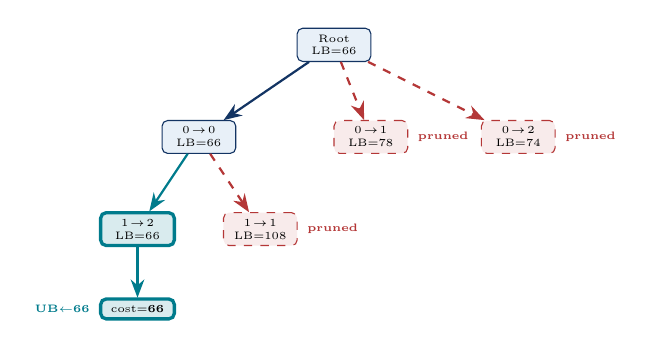
\begin{tikzpicture}[
    scale=0.78, transform shape,
    nd/.style={rectangle,rounded corners=2pt,draw=PrimaryBlue,fill=LightBG,
      font=\tiny,inner sep=3pt,align=center,minimum width=12mm},
    best/.style={nd,draw=Teal,fill=Teal!15,very thick},
    cut/.style={nd,draw=AlertRed,fill=AlertRed!10,dashed},
    >=Stealth,
  ]
  % Level 0 - Root
  \node[nd] (root) at (0,0) {Root\\LB=66};
  % Level 1
  \node[nd] (a) at (-2.2,-1.5) {$0\!\to\!0$\\LB=66};
  \node[cut] (b) at (0.6,-1.5) {$0\!\to\!1$\\LB=78};
  \node[cut] (c) at (3.0,-1.5) {$0\!\to\!2$\\LB=74};
  \draw[->,thick,PrimaryBlue] (root) -- (a);
  \draw[->,thick,AlertRed,dashed] (root) -- (b);
  \draw[->,thick,AlertRed,dashed] (root) -- (c);
  % Level 2 under 0->0
  \node[best] (ac) at (-3.2,-3.0) {$1\!\to\!2$\\LB=66};
  \node[cut] (ab) at (-1.2,-3.0) {$1\!\to\!1$\\LB=108};
  \draw[->,thick,Teal] (a) -- (ac);
  \draw[->,thick,AlertRed,dashed] (a) -- (ab);
  \node[font=\tiny\bfseries,AlertRed,right=1pt of ab] {pruned};
  % Level 3 leaf
  \node[best] (leaf1) at (-3.2,-4.3) {cost=\textbf{66}};
  \draw[->,thick,Teal] (ac) -- (leaf1);
  \node[font=\tiny\bfseries,Teal,left=1pt of leaf1] {UB$\leftarrow$66};
  % Pruned annotations
  \node[font=\tiny\bfseries,AlertRed,right=1pt of b] {pruned};
  \node[font=\tiny\bfseries,AlertRed,right=1pt of c] {pruned};
\end{tikzpicture}
\end{columns}

\vspace{4pt}
\begin{enumerate}\itemsep0pt
\item Root: LB=66, UB=$\infty$. Branch on facility 0.
\item Expand $0\!\to\!0$ (LB=66 $<$ UB). Child $1\!\to\!2$: LB=66, reach leaf $\pi\!=\!(0,2,1)$, cost=\alert{66}. UB$\leftarrow$66.
\item Child $1\!\to\!1$: LB=108 $\ge$ 66 $\Rightarrow$ \alert{pruned}.
\item $0\!\to\!1$: LB=78 $\ge$ 66 $\Rightarrow$ \alert{pruned}. \quad $0\!\to\!2$: LB=74 $\ge$ 66 $\Rightarrow$ \alert{pruned}.
\end{enumerate}
\textbf{Result:} Optimal $\pi^*\!=\!(0,2,1)$, cost \textbf{66}. Only 4 of 6 nodes explored.
\end{frame}

% ─── Slide 20: Robust Tabu Search ───────────────────────────────────────────
\begin{frame}{Algorithm 2: Robust Tabu Search}
\begin{block}{Concept}
\alert{Local Search} enhanced with \alert{short-term memory} (tabu list).
\end{block}
\vspace{4pt}
\begin{itemize}\setlength\itemsep{6pt}
  \item \textbf{State space:} permutations $\Sn$
  \item \textbf{Neighborhood:} 2-swap \quad $\pi' = \pi\circ(r,s)$
  \item \textbf{Neighborhood size:} $\binom{n}{2} = \BigO(n^2)$ neighbors
  \item \textbf{Challenge:} evaluating each neighbor na\"ively costs $\BigO(n^2)$ \\
        $\Rightarrow$ total per iteration: $\BigO(n^4)$
  \item \textbf{Key insight:} \alert{$\BigO(n)$ delta evaluation} using incremental formula
\end{itemize}
\vspace{4pt}
\reference{Taillard, \emph{EJOR}, 1991}
\end{frame}

% ─── Slide 20: Delta Evaluation ──────────────────────────────────────────────
\begin{frame}{$\BigO(n)$ Delta Evaluation}
Consider swapping positions $r$ and $s$. Let $p=\pi(r)$, $q=\pi(s)$.

\vspace{4pt}
\[
  \Delta(r,s) = \Delta^{\text{ext}} + \Delta^{\text{int}}
\]

\begin{block}{External part --- $\BigO(n)$}
\[
  \Delta^{\text{ext}} = \sum_{\substack{k=1\\k\neq r,s}}^{n}
  \bigl(F_{rk}-F_{sk}\bigr)\bigl(D_{q,\pi(k)}-D_{p,\pi(k)}\bigr)
  + \bigl(F_{kr}-F_{ks}\bigr)\bigl(D_{\pi(k),q}-D_{\pi(k),p}\bigr)
\]
\end{block}

\begin{block}{Internal part --- $\BigO(1)$}
\[
  \Delta^{\text{int}} =
  (F_{rs}-F_{sr})(D_{qp}-D_{pq})
\]
\end{block}

\textbf{Result:} Each swap evaluated in $\BigO(n)$ $\Rightarrow$ full neighborhood in $\BigO(n^3)$.

\reference{Taillard, 1991}
\end{frame}

% ─── Slide 21: Tabu Search Pseudocode ────────────────────────────────────────
\begin{frame}{Tabu Search --- Pseudocode}
\begin{block}{}
\small
\vspace{-2pt}
\begin{tabbing}
\hspace{4mm}\=\hspace{4mm}\=\hspace{4mm}\=\hspace{4mm}\=\kill
\textbf{Initialize:} random permutation $\pi$;\; $\pi^*\leftarrow\pi$\\[2pt]
\textbf{for} $t=1$ to $T$ \textbf{do}\\
\> $\text{BestSwap}\leftarrow\text{null}$\\
\> \textbf{for all} pairs $(r,s)$, $r<s$:\\
\>\> Compute $\Delta(r,s)$ in $\BigO(n)$\\
\>\> Check: is $(r,s)$ \alert{tabu}? Aspiration criterion?\\
\>\> \textbf{if} allowed \textbf{and} $\Delta<\Delta_{\text{best}}$:\\
\>\>\> $\text{BestSwap}\leftarrow(r,s)$\\[2pt]
\> Apply BestSwap to $\pi$\\
\> Update tabu list: mark $(r,s)$ tabu for $\tau$ iterations\\
\> \textbf{if} $\mathrm{Cost}(\pi)<\mathrm{Cost}(\pi^*)$:\\
\>\> $\pi^*\leftarrow\pi$\\[2pt]
\textbf{return} $\pi^*$
\end{tabbing}
\vspace{-4pt}
\end{block}
\vspace{2pt}
\textbf{Aspiration:} allow tabu move if it improves $\pi^*$.
\end{frame}

% ─── Slide 23: Tabu Search Walkthrough (NEW) ─────────────────────────────────
\begin{frame}[shrink=5]{Tabu Search Walkthrough: $n=4$ Example}
\small
\textbf{Instance:} 4 facilities, 4 locations.\quad
Start: $\pi=(1,2,3,4)$, Cost$\,{=}\,340$, tenure $\tau=2$.

\vspace{4pt}
\centering
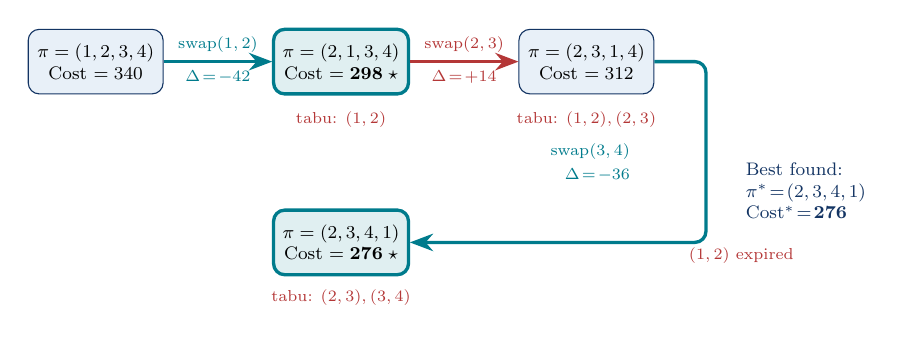
\begin{tikzpicture}[
    scale=0.82, transform shape,
    state/.style={rectangle,rounded corners=4pt,draw=PrimaryBlue,fill=LightBG,
      font=\footnotesize,inner sep=4pt,align=center,minimum width=2cm,minimum height=1cm},
    best/.style={state,draw=Teal,fill=Teal!12,very thick},
    lbl/.style={font=\scriptsize},
    >=Stealth,
  ]
  % State 0 (step 1)
  \node[state] (s0) at (0,0) {$\pi=(1,2,3,4)$\\Cost $= 340$};
  % State 1 (step 2)
  \onslide<2->{
    \node[best] (s1) at (3.8,0) {$\pi=(2,1,3,4)$\\Cost $= \mathbf{298}\;\star$};
    \draw[->,very thick,Teal] (s0) -- (s1)
      node[midway,above,lbl] {swap$(1,2)$}
      node[midway,below,lbl,Teal] {$\Delta\!=\!-42$};
    \node[lbl,AlertRed] at (3.8,-0.9) {tabu: $(1,2)$};
  }
  % State 2 (step 3)
  \onslide<3->{
    \node[state] (s2) at (7.6,0) {$\pi=(2,3,1,4)$\\Cost $= 312$};
    \draw[->,very thick,AlertRed] (s1) -- (s2)
      node[midway,above,lbl] {swap$(2,3)$}
      node[midway,below,lbl,AlertRed] {$\Delta\!=\!+14$};
    \node[lbl,AlertRed] at (7.6,-0.9) {tabu: $(1,2),(2,3)$};
  }
  % State 3 (step 4) — arrow routed right-down-left
  \onslide<4->{
    \node[best] (s3) at (3.8,-2.8) {$\pi=(2,3,4,1)$\\Cost $= \mathbf{276}\;\star$};
    \draw[->,very thick,Teal,rounded corners=4pt] (s2.east) -- ++(0.8,0) -- ++(0,-2.8) -- (s3.east);
    \node[lbl,Teal,left] at (8.4,-1.4) {swap$(3,4)$};
    \node[lbl,Teal,left] at (8.4,-1.75) {$\Delta\!=\!-36$};
    \node[lbl,AlertRed] at (3.8,-3.65) {tabu: $(2,3),(3,4)$};
    % Best annotation - far right
    \node[font=\footnotesize,PrimaryBlue,align=left] at (11.0,-2.0) {%
      Best found:\\
      $\pi^*\!=\!(2,3,4,1)$\\
      Cost$^*\!=\!\mathbf{276}$};
    \node[lbl,AlertRed] at (10.0,-3.0) {$(1,2)$ expired};
  }
\end{tikzpicture}

\vspace{4pt}
\begin{columns}[T]
\column{0.48\textwidth}
\textbf{Key observations:}
\begin{itemize}\itemsep1pt
  \item Iter 2: \alert{accepted worsening move} ($+14$) --- best non-tabu option
  \item Escapes the local optimum at 298
  \item Iter 3: new global best 276
\end{itemize}
\column{0.48\textwidth}
\textbf{Tabu list dynamics:}
\begin{itemize}\itemsep1pt
  \item After swap$(r,s)$: reverse forbidden for $\tau\!=\!2$ iterations
  \item Prevents cycling back immediately
  \item $(1,2)$ expired after iter 3
  \item $\star$ = new global best
\end{itemize}
\end{columns}
\end{frame}

% =============================================================================
%  PART 5: Proposed Modifications
% =============================================================================

% ─── Slide 22: B&B Mod 1 — Greedy Initial UB ────────────────────────────────
\begin{frame}{B\&B Modification 1: Greedy Initial Upper Bound}
\begin{alertblock}{Problem}
Starting with $\mathrm{UB}=+\infty$ means \alert{no pruning} in early iterations.
\end{alertblock}
\vspace{4pt}
\begin{block}{Solution: Greedy Heuristic}
Before B\&B, compute an initial solution:
\begin{enumerate}
  \item Rank facilities by total flow: $\sum_j F_{ij}$ (descending)
  \item Rank locations by total distance: $\sum_\ell D_{k\ell}$ (ascending)
  \item Assign highest-flow facility to lowest-distance location
\end{enumerate}
\end{block}
\vspace{4pt}
\textbf{Effect:} Tighter initial UB $\Rightarrow$ earlier pruning $\Rightarrow$ \alert{fewer nodes explored}.

\reference{Loiola et al., \emph{EJOR}, 2007}
\end{frame}

% ─── Slide 23: B&B Mod 2 — LB-Ordered Children ──────────────────────────────
\begin{frame}{B\&B Modification 2: LB-Ordered Child Exploration}
\begin{columns}[T]
\column{0.52\textwidth}
\begin{alertblock}{Problem}
DFS explores children in arbitrary order; a bad branch is expanded before a promising one.
\end{alertblock}
\vspace{4pt}
\begin{block}{Solution}
Before pushing children onto the DFS stack, \alert{sort by LB ascending}.\\
\smallskip
Lowest-LB child is pushed \emph{last} $\Rightarrow$ popped \emph{first}.
\end{block}
\vspace{4pt}
\textbf{Trade-off:}
\begin{itemize}
  \item[\textcolor{Teal}{+}] Steers DFS toward the optimum earlier
  \item[\textcolor{Teal}{+}] Same $\mathcal{O}(n)$ memory as plain DFS
  \item[\textcolor{AlertRed}{--}] Extra LB computation per child
\end{itemize}

\column{0.45\textwidth}
\centering
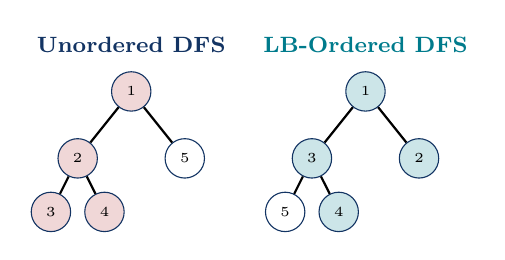
\begin{tikzpicture}[
    tnode/.style={circle,draw=PrimaryBlue,minimum size=5mm,font=\tiny},
    scale=0.85,
    >=Stealth
  ]
  % Unordered DFS tree
  \node[font=\footnotesize\bfseries,PrimaryBlue] at (0,2.5) {Unordered DFS};
  \node[tnode,fill=AlertRed!20] (a) at (0,1.8) {1};
  \node[tnode,fill=AlertRed!20] (b) at (-0.8,0.8) {2};
  \node[tnode] (c) at (0.8,0.8) {5};
  \node[tnode,fill=AlertRed!20] (d) at (-1.2,0) {3};
  \node[tnode,fill=AlertRed!20] (e) at (-0.4,0) {4};
  \draw[thick] (a)--(b) (a)--(c) (b)--(d) (b)--(e);

  % LB-ordered DFS tree
  \node[font=\footnotesize\bfseries,Teal] at (3.5,2.5) {LB-Ordered DFS};
  \node[tnode,fill=Teal!20] (a2) at (3.5,1.8) {1};
  \node[tnode,fill=Teal!20] (b2) at (2.7,0.8) {3};
  \node[tnode,fill=Teal!20] (c2) at (4.3,0.8) {2};
  \node[tnode] (d2) at (2.3,0) {5};
  \node[tnode,fill=Teal!20] (e2) at (3.1,0) {4};
  \draw[thick] (a2)--(b2) (a2)--(c2) (b2)--(d2) (b2)--(e2);
\end{tikzpicture}
{\scriptsize Numbers indicate visit order}
\end{columns}
\end{frame}

% ─── Slide 24: TS Mod 1 — Reactive Tenure ───────────────────────────────────
\begin{frame}{Tabu Search Modification: Reactive Tenure}
\begin{alertblock}{Problem}
Fixed tenure $\tau$ may be \alert{too short} (cycling) or \alert{too long} (slow exploration).
\end{alertblock}
\vspace{4pt}
\begin{block}{Solution: Dynamic Tenure}
Adapt $\tau$ based on search history using solution hashing:
\begin{itemize}
  \item If a solution is \alert{revisited} (hash collision detected):
        \[\tau \leftarrow \tau \times 1.1 \qquad\text{(increase to escape cycle)}\]
  \item Otherwise, slowly decay toward baseline:
        \[\tau \leftarrow \tau \times 0.995 \qquad\text{(allow exploitation)}\]
\end{itemize}
\end{block}
\vspace{2pt}
\textbf{Baseline:} $\tau_0 = \lfloor n/4\rfloor$.\quad
\textbf{Bounds:} $\tau\in[1,\,n]$.

\reference{Battiti \& Tecchiolli, \emph{ORSA J.\ Comp.}, 1994}
\end{frame}

% ─── Slide 25: TS Mod 2 — Diversification Restarts ──────────────────────────
\begin{frame}{Tabu Search Modification: Diversification Restarts}
\begin{alertblock}{Problem}
Search may \alert{stagnate} in a region with no improving moves for many iterations.
\end{alertblock}
\vspace{4pt}
\begin{block}{Solution: Perturbation-Based Restart}
After $10n$ non-improving iterations:
\begin{enumerate}
  \item Return to the best-known solution $\pi^*$
  \item Apply 3 random swaps to perturb it
  \item Resume tabu search from the perturbed solution
  \item Reset the tabu list
\end{enumerate}
\end{block}
\vspace{4pt}
Combined with reactive tenure $\Rightarrow$ more \alert{robust exploration}.\\
This is an instance of the \emph{Iterated Local Search} (ILS) paradigm.

\reference{St\"utzle, 2006; Louren\c{c}o et al., ILS+TS}
\end{frame}

% =============================================================================
%  PART 6: Experimental Results
% =============================================================================

% ─── Slide 26: Experimental Setup ───────────────────────────────────────────
\begin{frame}{Experimental Setup}
\begin{columns}[T]
\column{0.48\textwidth}
\begin{block}{Datasets}
\begin{itemize}
  \item \textbf{QAPLIB} benchmark instances
  \item Families: \texttt{nug}, \texttt{chr}, \texttt{tai}
  \item $n\in\{12,14,15,20,25,30\}$
  \item Best-known solutions (BKS) from QAPLIB
\end{itemize}
\end{block}
\begin{block}{Metrics}
\begin{itemize}
  \item Runtime (seconds)
  \item Memory usage (MB)
  \item Nodes explored (B\&B)
  \item Solution quality (Gap\%)
\end{itemize}
\end{block}

\column{0.48\textwidth}
\begin{block}{Protocol}
\begin{itemize}
  \item B\&B: $n\le 14$ with 60\,s timeout
  \item Tabu Search: all sizes, $T=\max(3000,\,150n)$
\end{itemize}
\end{block}
\begin{block}{Environment}
\begin{itemize}
  \item Hardware: standard laptop
  \item Python 3 with NumPy, SciPy
  \item Plots via Matplotlib
\end{itemize}
\end{block}
\end{columns}
\vspace{4pt}
\reference{QAPLIB: Burkard, Karisch \& Rendl, 1997}
\end{frame}

% ─── Slide 27: B&B Runtime Comparison ────────────────────────────────────────
\begin{frame}{B\&B Runtime Comparison}
\begin{columns}[c]
\column{0.65\textwidth}
\centering

\includegraphics[width=0.85\linewidth]{plots/bb_runtime_vs_n.pdf}
\column{0.33\textwidth}
\begin{block}{Observations}
\begin{itemize}
  \item Log-scale $y$-axis
  \item Improved B\&B (greedy UB + LB-ordered DFS) shows \alert{faster convergence}
  \item Greedy initialization provides a tighter starting bound
\end{itemize}
\end{block}
\end{columns}
\end{frame}

% ─── Slide 28: B&B Nodes Explored ───────────────────────────────────────────
\begin{frame}{B\&B Nodes Explored}
\begin{columns}[c]
\column{0.65\textwidth}
\centering

\includegraphics[width=0.85\linewidth]{plots/bb_nodes_explored.pdf}
\column{0.33\textwidth}
\begin{block}{Observations}
\begin{itemize}
  \item Greedy upper bound \alert{dramatically reduces} nodes explored
  \item LB-ordered child expansion focuses DFS on promising branches
  \item Combined effect: \alert{9--34$\times$} fewer nodes explored
\end{itemize}
\end{block}
\end{columns}
\end{frame}

% ─── Slide 29: TS Convergence ────────────────────────────────────────────────
\begin{frame}{Tabu Search Convergence}
\begin{columns}[c]
\column{0.65\textwidth}
\centering

\includegraphics[width=0.85\linewidth]{plots/ts_convergence.pdf}
\column{0.33\textwidth}
\begin{block}{Observations (chr15a)}
\begin{itemize}
  \item TS-Original \alert{stagnates} at iteration~100
  \item TS-Reactive keeps improving via dynamic tenure and diversification
  \item Final gap: TS-Original 31.6\% vs TS-Reactive \alert{0.83\%}
\end{itemize}
\end{block}
\end{columns}
\end{frame}

% ─── Slide 30: TS Gap Comparison ─────────────────────────────────────────────
\begin{frame}{Tabu Search --- Gap Comparison}
\begin{columns}[c]
\column{0.65\textwidth}
\centering

\includegraphics[width=0.85\linewidth]{plots/ts_gap_comparison.pdf}
\column{0.33\textwidth}
\begin{block}{Observations}
\begin{itemize}
  \item Gap\% = $\frac{\text{found}-\text{best known}}{\text{best known}}\times 100$
  \item Reactive TS achieves \alert{lower gap\%} on most instances
  \item Largest improvement: chr15a (31.6\% $\to$ 0.83\%); consistently better at $n\le 20$
\end{itemize}
\end{block}
\end{columns}
\end{frame}

% ─── Slide 31: TS Runtime vs Problem Size ────────────────────────────────────
\begin{frame}{Tabu Search --- Runtime Scalability}
\begin{columns}[c]
\column{0.65\textwidth}
\centering

\includegraphics[width=0.85\linewidth]{plots/ts_runtime_vs_n.pdf}
\column{0.33\textwidth}
\begin{block}{Observations}
\begin{itemize}
  \item TS scales from $n=12$ to $n=30$ without timeout
  \item Runtime grows as $\mathcal{O}(n^3)$--$\mathcal{O}(n^4)$: $n{=}12\to10\,\text{s}$, $n{=}30\to274\,\text{s}$
  \item TS-Reactive overhead is negligible ($<$1\% vs Original)
  \item Unlike B\&B, TS completes all instances
\end{itemize}
\end{block}
\end{columns}
\end{frame}

% ─── Slide 32: Memory Usage ─────────────────────────────────────────────────
\begin{frame}{Memory Usage Comparison}
\begin{columns}[c]
\column{0.65\textwidth}
\centering

\includegraphics[width=0.85\linewidth]{plots/memory_comparison.pdf}
\column{0.33\textwidth}
\begin{block}{Observations}
\begin{itemize}
  \item TS-Reactive uses most memory due to visited-solution hash set (up to 0.30\,MB)
  \item B\&B variants use negligible memory ($<$0.02\,MB) with DFS stack
  \item Tabu Search is \alert{memory-efficient}: $\BigO(n^2)$ for matrices + $\BigO(n)$ for tabu list
  \item Trade-off: memory vs.\ optimality guarantee
\end{itemize}
\end{block}
\end{columns}
\end{frame}

% ─── Slide 33: Overall Algorithm Comparison ──────────────────────────────────
\begin{frame}{Overall Algorithm Comparison}
\begin{columns}[c]
\column{0.65\textwidth}
\centering

\includegraphics[width=0.85\linewidth]{plots/algorithm_comparison.pdf}
\column{0.33\textwidth}
\begin{block}{Observations}
\begin{itemize}
  \item TS-Reactive finds \alert{optimal} on all 4 instances; B\&B on 3 of 4 (nug14 timeout)
  \item B\&B hits timeout for $n\ge 12$; TS scales to $n=30$
\end{itemize}
\end{block}
\end{columns}
\end{frame}

% ─── Slide 34: Results Summary Table ─────────────────────────────────────────
\begin{frame}[shrink=5]{Results Summary}
\centering
\small
\begin{tabular}{@{}l c r rr rr r@{}}
\toprule
 & & & \multicolumn{2}{c}{\textbf{B\&B Orig.}} &
      \multicolumn{2}{c}{\textbf{B\&B Impr.}} &
      \textbf{TS React.}\\
\cmidrule(lr){4-5}\cmidrule(lr){6-7}\cmidrule(lr){8-8}
\textbf{Instance} & $n$ & \textbf{BKS} & Cost & Time & Cost & Time & Gap\,\%\\
\midrule
nug12  & 12 & 578     & \textbf{578}    & T/O   & \textbf{578}   & T/O  & \textbf{0.00}\\
chr12a & 12 & 9552    & \textbf{9552}   & 5.7   & \textbf{9552} & 1.2  & \textbf{0.00}\\
tai12a & 12 & 224416  & \textbf{224416} & 56.1  & \textbf{224416} & 30.0 & \textbf{0.00}\\
nug14  & 14 & 1014    & 1030            & T/O   & \textbf{1022}  & T/O  & \textbf{0.00}\\
chr15a & 15 & 9896    & ---             & ---   & ---        & ---  & 0.83\\
tai15a & 15 & 388214  & ---             & ---   & ---        & ---  & \textbf{0.00}\\
nug20  & 20 & 2570    & ---             & ---   & ---        & ---  & \textbf{0.00}\\
tai20a & 20 & 703482  & ---             & ---   & ---        & ---  & 0.67\\
nug25  & 25 & 3744    & ---             & ---   & ---        & ---  & \textbf{0.00}\\
tai25a & 25 & 1167256 & ---             & ---   & ---        & ---  & 1.43\\
nug30  & 30 & 6124    & ---             & ---   & ---        & ---  & 0.62\\
tai30a & 30 & 1818146 & ---             & ---   & ---        & ---  & 0.39\\
\bottomrule
\end{tabular}
\vspace{4pt}

{\footnotesize T/O = timeout (60\,s). Bold = optimal found. BKS from QAPLIB (Burkard et al., 1997).\\
B\&B Improved: greedy UB + LB-ordered DFS. On chr12a: \alert{$5\times$ speedup} (5.7\,s $\to$ 1.2\,s); on nug14: better solution under timeout (1022 vs 1030).\\
TS Reactive finds BKS on 7 of 12 instances.}
\end{frame}

% =============================================================================
%  PART 7: Closing
% =============================================================================

% ─── Slide 35: Real-World Applications ───────────────────────────────────────
\begin{frame}{Real-World Applications}
\begin{columns}[T]
\column{0.32\textwidth}
\centering

\begin{tikzpicture}
  \draw[PrimaryBlue,fill=LightBG,rounded corners,thick] (-0.6,-0.6) rectangle (0.6,0.6);
  \draw[PrimaryBlue,thick] (-0.3,-0.4) rectangle (-0.05,0.3);
  \draw[PrimaryBlue,thick] (0.05,-0.4) rectangle (0.3,0.3);
  \draw[PrimaryBlue,thick] (-0.3,0.3) -- (-0.17,0.5) -- (0.17,0.5) -- (0.3,0.3);
\end{tikzpicture}
\vspace{2pt}

\textbf{Facility \& Campus Layout}
\vspace{4pt}

\small
$F_{ij}$: material flow\\
$D_{k\ell}$: physical distance\\[4pt]
Minimize transport cost between departments.

\column{0.32\textwidth}
\centering

\begin{tikzpicture}
  \draw[Teal,fill=LightBG,rounded corners,thick] (-0.6,-0.6) rectangle (0.6,0.6);
  \draw[Teal,thick] (-0.35,-0.35) grid[step=0.23] (0.35,0.35);
  \fill[Teal] (-0.12,-0.12) rectangle (0.12,0.12);
\end{tikzpicture}
\vspace{2pt}

\textbf{VLSI \& Chip Design}
\vspace{4pt}

\small
$F_{ij}$: net connectivity\\
$D_{k\ell}$: Manhattan distance\\[4pt]
Minimize total wire length on chip.

\column{0.32\textwidth}
\centering

\begin{tikzpicture}
  \draw[Gold!80!black,fill=LightBG,rounded corners,thick] (-0.7,-0.4) rectangle (0.7,0.4);
  \foreach \x in {-0.5,-0.25,0,0.25,0.5} {
    \draw[Gold!80!black,thick] (\x,-0.05) rectangle ++(0.15,0.15);
  }
  \foreach \x in {-0.5,-0.25,0,0.25,0.5} {
    \draw[Gold!80!black,thick] (\x,-0.25) rectangle ++(0.15,0.15);
  }
  \draw[Gold!80!black,thick] (-0.3,0.15) rectangle ++(0.75,0.15);
\end{tikzpicture}
\vspace{2pt}

\textbf{Keyboard Layout}
\vspace{4pt}

\small
$F_{ij}$: digram frequency\\
$D_{k\ell}$: finger travel distance\\[4pt]
Minimize total typing effort.
\end{columns}
\end{frame}

% ─── Slide 36: Reproducibility ──────────────────────────────────────────────
\begin{frame}{Reproducibility}
\begin{block}{Code Repository}
All source code available at \url{https://github.com/Tausif-Rashid/CSE462_Algorithm_Project}
\end{block}
\vspace{6pt}
\begin{block}{Master Script}
\texttt{\$ python main.py}
\begin{itemize}
  \item Uses QAPLIB benchmark instances
  \item Runs all algorithm variants (B\&B original, B\&B improved, TS original, TS reactive)
  \item Collects timing and quality metrics
  \item Produces all plots as PDF in \texttt{plots/}
\end{itemize}
\end{block}
\vspace{4pt}
\begin{block}{Requirements}
Python~3, NumPy, SciPy, Matplotlib
\end{block}
\end{frame}

% ─── Slide 37: Key Takeaways ────────────────────────────────────────────────
\begin{frame}{Key Takeaways}
\begin{enumerate}\setlength\itemsep{10pt}
  \item \textbf{QAP is NP-Hard} --- proved via reductions from both
        \alert{Symmetric TSP} and \alert{Balanced Cut}

  \item \textbf{Branch-and-Bound} gives \alert{optimal} solutions
        but is limited to small instances ($n\le 14$ within 60\,s)

  \item \textbf{Tabu Search} scales well to $n=30+$;
        \alert{reactive tenure} and \alert{diversification restarts}
        improve solution quality

  \item \textbf{Proposed modifications} show measurable improvement:
        \begin{itemize}
          \item Greedy UB + LB-ordered DFS: 9--34$\times$ fewer nodes, $5\times$ speedup on chr12a
          \item Better solution under timeout on nug14 (1022 vs 1030)
          \item Reactive tenure: lower gap\% on most instances
        \end{itemize}
\end{enumerate}
\end{frame}

% ─── Slide 38: References ───────────────────────────────────────────────────
\begin{frame}{References}
\small
\begin{enumerate}
  \item Koopmans, T.C.\ \& Beckmann, M.\ (1957).
        Assignment problems and the location of economic activities.
        \emph{Econometrica}, 25(1), 53--76.
  \item Gilmore, P.C.\ (1962).
        Optimal and suboptimal algorithms for the quadratic assignment problem.
        \emph{SIAM Journal}, 10(2), 305--313.
  \item Lawler, E.L.\ (1963).
        The quadratic assignment problem.
        \emph{Management Science}, 9(4), 586--599.
  \item Glover, F.\ (1989, 1990).
        Tabu search.
        \emph{ORSA Journal on Computing}, 1(3), 190--206; 2(1), 4--32.
  \item Taillard, \'E.\ (1991).
        Robust taboo search for the QAP.
        \emph{Parallel Computing}, 17, 443--455.
  \item Battiti, R.\ \& Tecchiolli, G.\ (1994).
        The reactive tabu search.
        \emph{ORSA Journal on Computing}, 6(2), 126--140.
  \item Burkard, R.E., Karisch, S.E.\ \& Rendl, F.\ (1997).
        QAPLIB --- A quadratic assignment problem library.
        \emph{JGLO}, 10, 391--403.
  \item Loiola, E.M.\ et al.\ (2007).
        A survey for the quadratic assignment problem.
        \emph{EJOR}, 176(2), 657--690.
\end{enumerate}
\end{frame}

% ─── Slide 39: Thank You ────────────────────────────────────────────────────
{
\setbeamercolor{background canvas}{bg=PrimaryBlue}
\begin{frame}[plain]
\centering
\vspace{1.5cm}
{\Huge\bfseries\textcolor{white}{Thank You!}}\\[20pt]
{\Large\textcolor{Gold}{Questions?}}\\[30pt]
{\small\textcolor{white}{%
  Md.\ Jakaria Hossain \quad
  Musa Tur Farazi \quad
  Md.\ As-Aid Rahman\\[4pt]
  MD Sajid Mostafiz Noor \quad
  Tausif Rashid \quad
  Awesh Islam\\[12pt]
  CSE 462 --- Algorithm Engineering Lab\\
  March 2026
}}
\end{frame}
}

\end{document}
